\documentclass{article}
\usepackage[utf8]{inputenc}
\usepackage{graphicx}
\usepackage{float}
\graphicspath{ {Diagrams/} }


\title{ Architectural Requirements Specifications and Design \\[0.5cm] 
\includegraphics[width=6cm]{front-page}}
\author{Andrew le Roux \hfill 15311644 \\ Cian Steenkamp \hfill 15095682 \\ Darren Adams \hfill 14256232 \\ Drew Langley \hfill [Student Number] \\ Martha Mohlala \hfill [Student Number] \\ Nsovo Baloyi \hfill 12163262 \\ Rikard Schouwstra \hfill [Student Number]}
\date{March 2017}
\begin{document}
\maketitle
\pagebreak
\tableofcontents
\pagebreak

\section{External Interface Requirements}
    \subsection{User Interfaces}
        The mobile application will interface with the supported input and output
        features of the host's operating system. Inputs include text that the user
        will enter for login or searching a venue. Outputs include the type of fonts
        to display text or graphics to show images or draw the map.

    \subsection{Hardware Interfaces}
        Since neither the mobile application nor the web portal have any designated
        hardware, it does not have any direct hardware interfaces. The WiFi software
        in the mobile phone manages the built-in WiFi and the hardware connection
        to the database server is managed by the underlying operating system on the
        mobile phone and the web server.

    \subsection{Software Interfaces}
        The mobile application communicates with the WiFi software in order to get
        signal strength information from multiple WiFi access points to determine
        (using triangulation) where the user is located. The communication software
        between the database and mobile application consists of operation concerning
        creating, reading, removing and modifying the data.

    \subsection{Communication Interfaces}
        The communication between the different parts of the system are important since they depend on each other. However, in what way the communication is achieved is not important for the system and is therefore handled by the underlying operating systems for both the mobile application and the back-end of the system.

\section{Performance Requirements}
\subsection{Performance}
\begin{itemize}
\item Offline activities should have a response time of +/- 2 seconds (instantaneous) when responding to an activity, while online activities such as calculating routes should have a response time of +/- 2-4 seconds so that the users have an uninterrupted experience.\\
\item It should also allow the integration of a variety of services.\\
\end{itemize}
\subsection{Reliability} 
\begin{itemize}
\item It should be able to handle +/- 50 000 users concurrently (simultaneously) when implemented into a suitable production environment. \\
 \item The application should be reliable, in that it will provide the fastest route every time without fail and complete all other computations successfully. \\
\item All activities should be completed with a 0.1 error allowance.\\
\item The application should provide accurate locations in a constantly changing environment.\\
\end{itemize}
\subsection{Security}
\begin{itemize}
\item Data transmission should be securely transmitted without unauthorized access, or loss of information.\\
\end{itemize}

\section{Design Constraints}

- The system should be accessible on smart devices, such as Android and iOS devices.\\
- The system should not use GPS, but only the WiFi network. \\
- The proposed system should be able to be integrated into the Computer Science Department's Web site. \\
- The system should be a modular system, to reduce the dependencies in the system. \\
- Software Fault Tolerance: If a malfunction cannot be avoided, then the software design should be constrained so that the system can recover without causing damage to the system. \\
- The system should have an aesthetically pleasing and easy to use interface. \\
- The system must be able to run on smart devices which has limited processing power, battery life and storage space. The system must thus use resources efficiently. \\
- The system needs to use open source technologies. \\


\section{System Software Attributes}

    \subsection{Reliability}
        
        \begin{description}
        
        \item[$\bullet$] Any information that is stored on the database must remain correct when being transferred to the user interface.
        \item[$\bullet$] The services offered by the system should be available to users except for when the system is undergoing maintenance.
        \item[$\bullet$] The system should reply to user requests in the shortest time interval possible.
        \item[$\bullet$] The system must be fault tolerant, it needs to maintain a certain level of performance and offer other services that are not affected by this fault to the users.
        \item[$\bullet$] In the event of a fault the system must be able to recover within the shortest time period possible and recover any data that may have been lost.
        \item[$\bullet$] The system should be able to respond appropriately if it receives bad input data from the user.
        
        \end{description}
        
    \subsection{Scalability}
    
        \begin{description}
    
        \item[$\bullet$] The system must be able to cater for increases in the work load, for example large number of users or activities at any given time, without impacting the performance of the system. 
        \item[$\bullet$] If the system does not cater for increases in workload it should at least provide the ability to be readily enlarged.
        
        \end{description}
    
    \subsection{Maintainability}
    
        \begin{description}
    
        \item[$\bullet$] The system must be designed in a modular fashion that provides high cohesion and loose coupling, this will allow parts of the system to be easily maintained without affecting the rest of the system.
        \item[$\bullet$]Maintenance should be able to be carried out by different maintenance teams, therefore the system must be easy to learn and understand.
        
        \end{description}
    
    \subsection{Integrability}
    
        \begin{description}
        
        \item[$\bullet$] Since we are following a modular design, components of the system that are separately developed should work correctly together.
        \item[$\bullet$] Follow coding standards specified by the client to allow for easy integration and employ continuous integration in our design process.
        
        \end{description}
    
    \subsection{Usability}
    
        \begin{description}
        
        \item[$\bullet$] The system must be easy to learn.
        \item[$\bullet$]System must cater for user mistakes, by providing the user with the undo or roll back options.
        \item[$\bullet$]The user interface must be easy to use and must be intuitive.
        \item[$\bullet$]The system should display options in a logical manner.
        \item[$\bullet$]Incorporate widgets and icons that the target users may be familiar with.
        \item[$\bullet$]The user manual should have a detailed description of the system.
        \item[$\bullet$]A help option must be provided to the users.
        
        \end{description}
    
    \subsection{Interoperability}
    
        \begin{description}
        
        \item[$\bullet$]The system must be able to communicate with the University of Pretoria WiFi system, because the WiFi  access points will be used for the navigation.
        
        \end{description}

\section{Modules}
	
	\subsection{Overview of System}
	\begin{figure}[H]
  	\caption{Deployment Diagram}
  	\centering
    	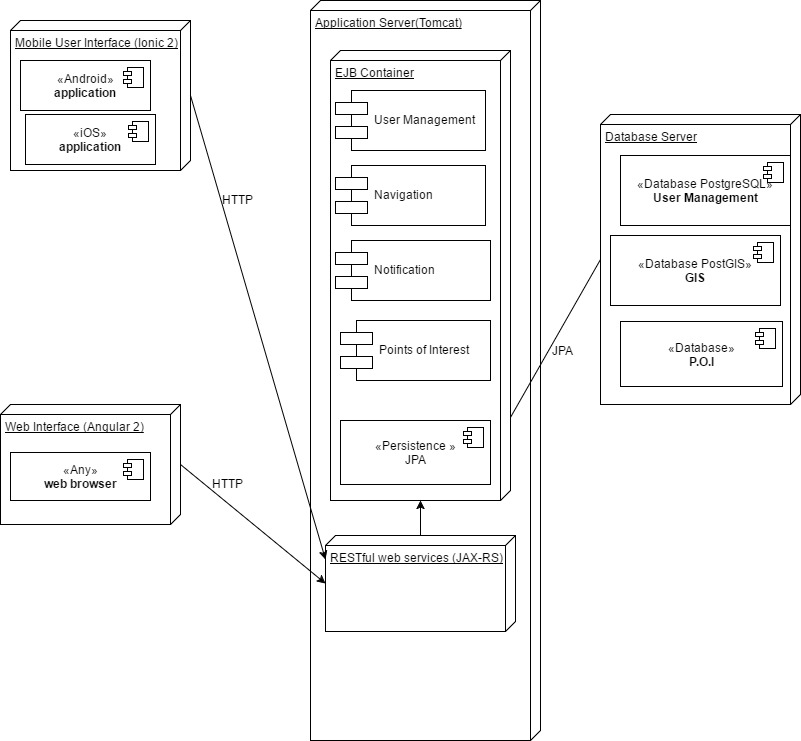
\includegraphics[width=8cm]{DeploymentDiagram}
\end{figure}

The figure above shows the deployment diagram. It show the various deployments of the components as well as the technologies to be used.\\[0.2cm]
The system will implement a layered architectural pattern. This allows us to separate the user interfaces from the business processes as well as the database services. It adds flexibly and maintainability to the system.\\[0.2cm]
The backend systems will be deployed on a JavaEE application server. Other devices may communicate with the server through an API there by implementing a façade. The web interface will run on any web browser and the mobile interface will be accessible on iOS and Android.
    \subsection{User Management}
        \subsubsection{Class Diagram}
        \subsubsection{Use Case Diagrams}
        \subsubsection{Other Diagrams}
        \subsubsection{Chosen Design Patterns}
    \subsection{Notifications}
        \subsubsection{Class Diagram}
    			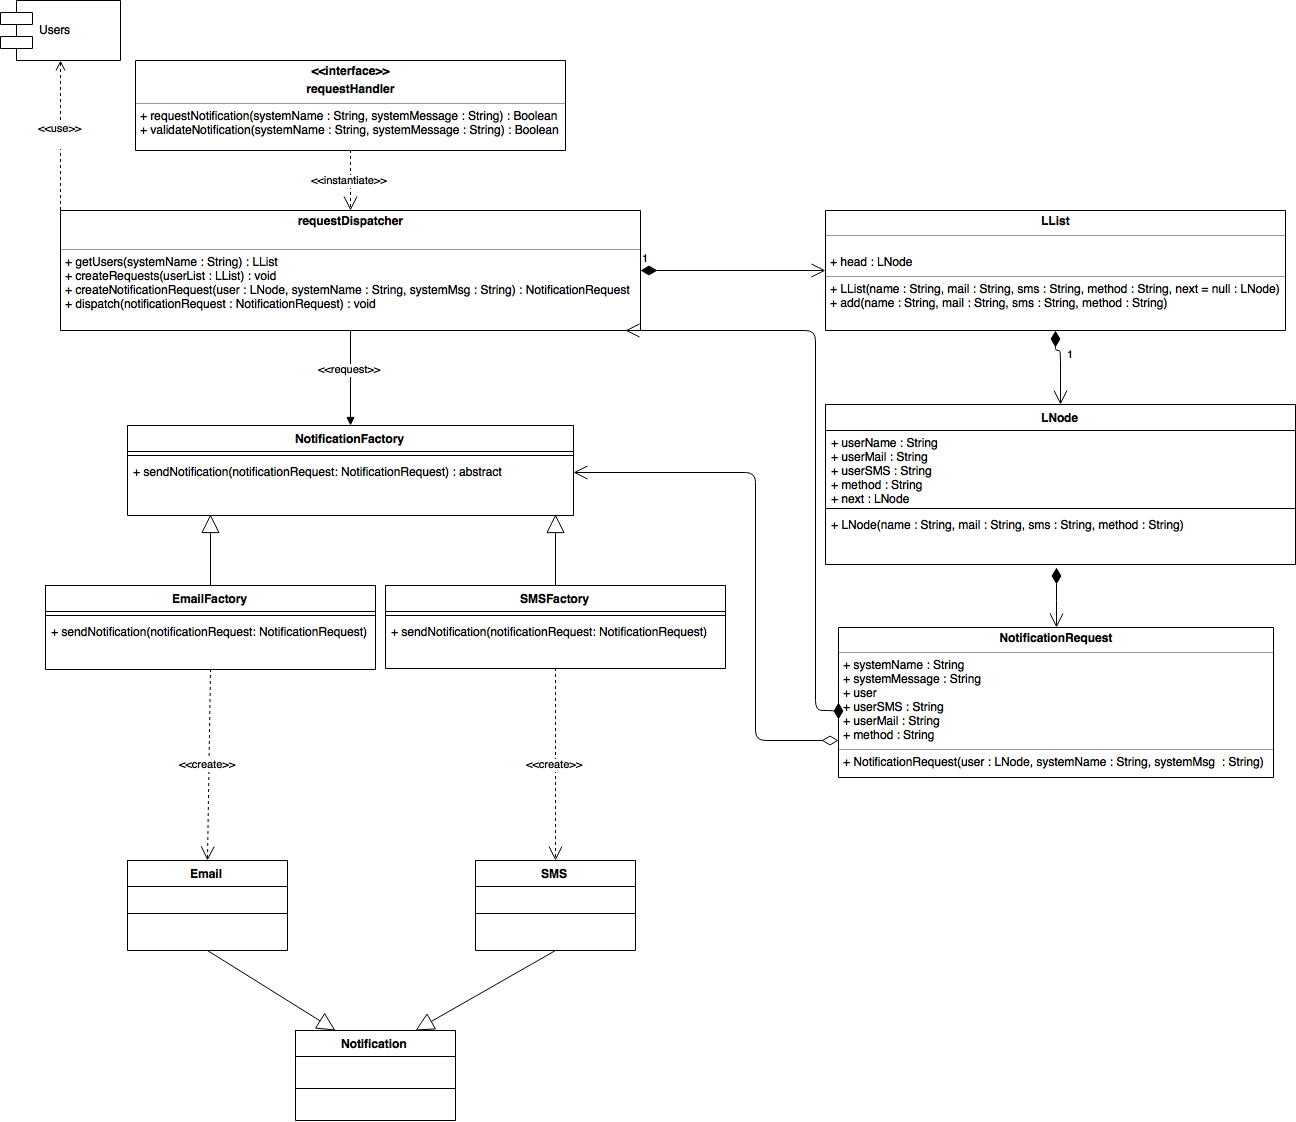
\includegraphics[width=0.5\textwidth]{Notifications_Class_Diagram}
        \subsubsection{Use Case Diagrams}
    			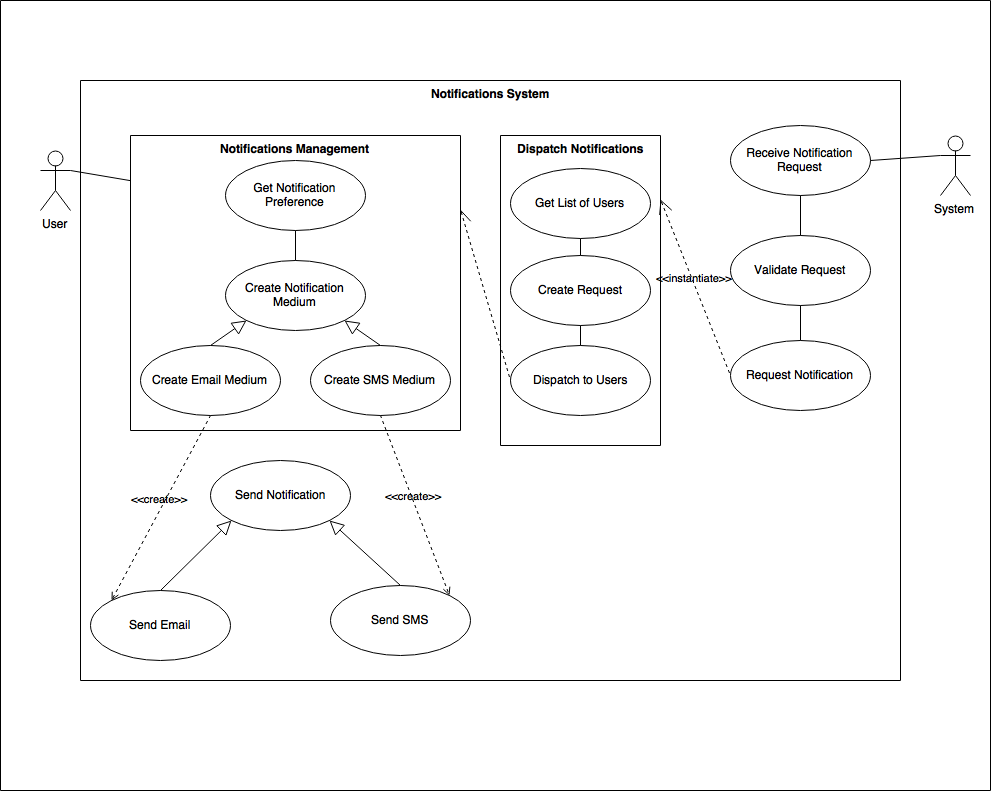
\includegraphics[width=0.5\textwidth]{NotificationUseCases}	
        \subsubsection{Chosen Design Patterns}
    \subsection{Navigation}
        \subsubsection{Class Diagram}
        \begin{figure}[H]
        	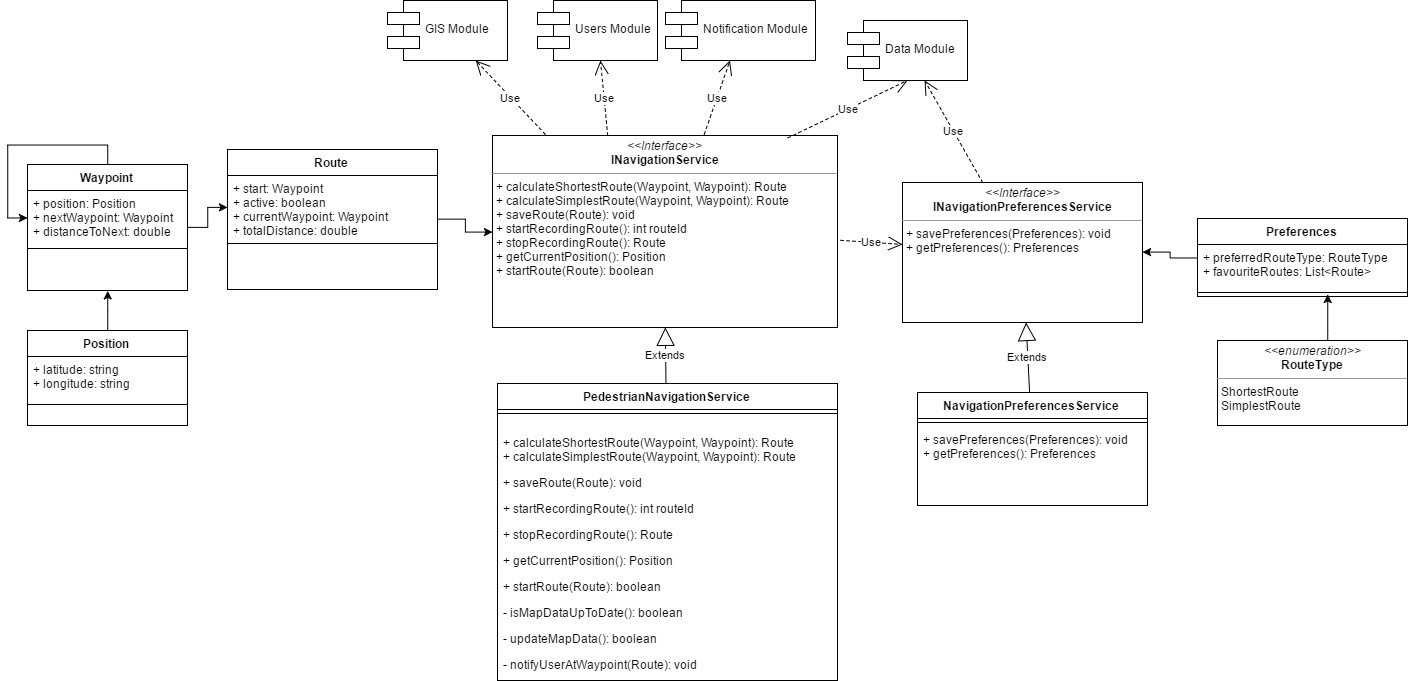
\includegraphics[width=\textwidth]{Navigation_Class_Diagram}
            \caption{Navigation Module Class Diagram}
        \end{figure}
        \subsubsection{Use Case Diagrams}
        \begin{figure}[H]
        	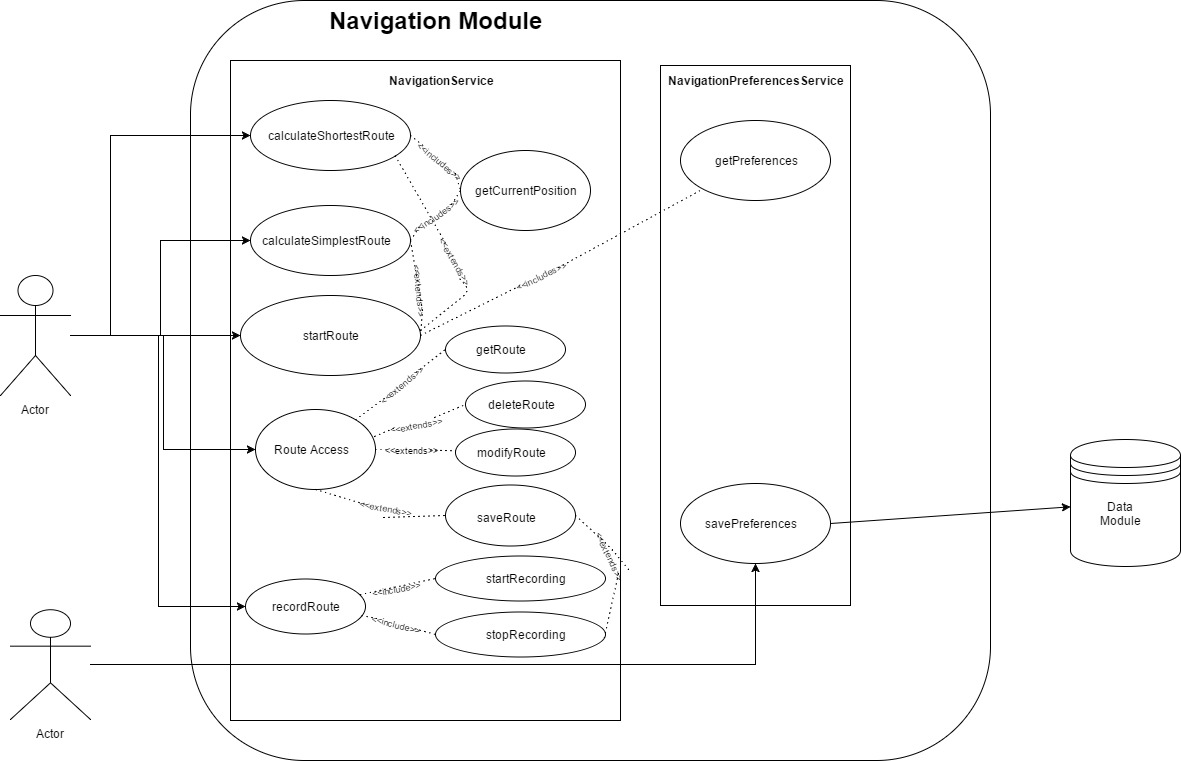
\includegraphics[width=\textwidth]{Navigation_Use_Case_Diagram}
            \caption{Navigation Module Use Case Diagram}
        \end{figure}
        \subsubsection{Other Diagrams}
        \begin{figure}[H]
        	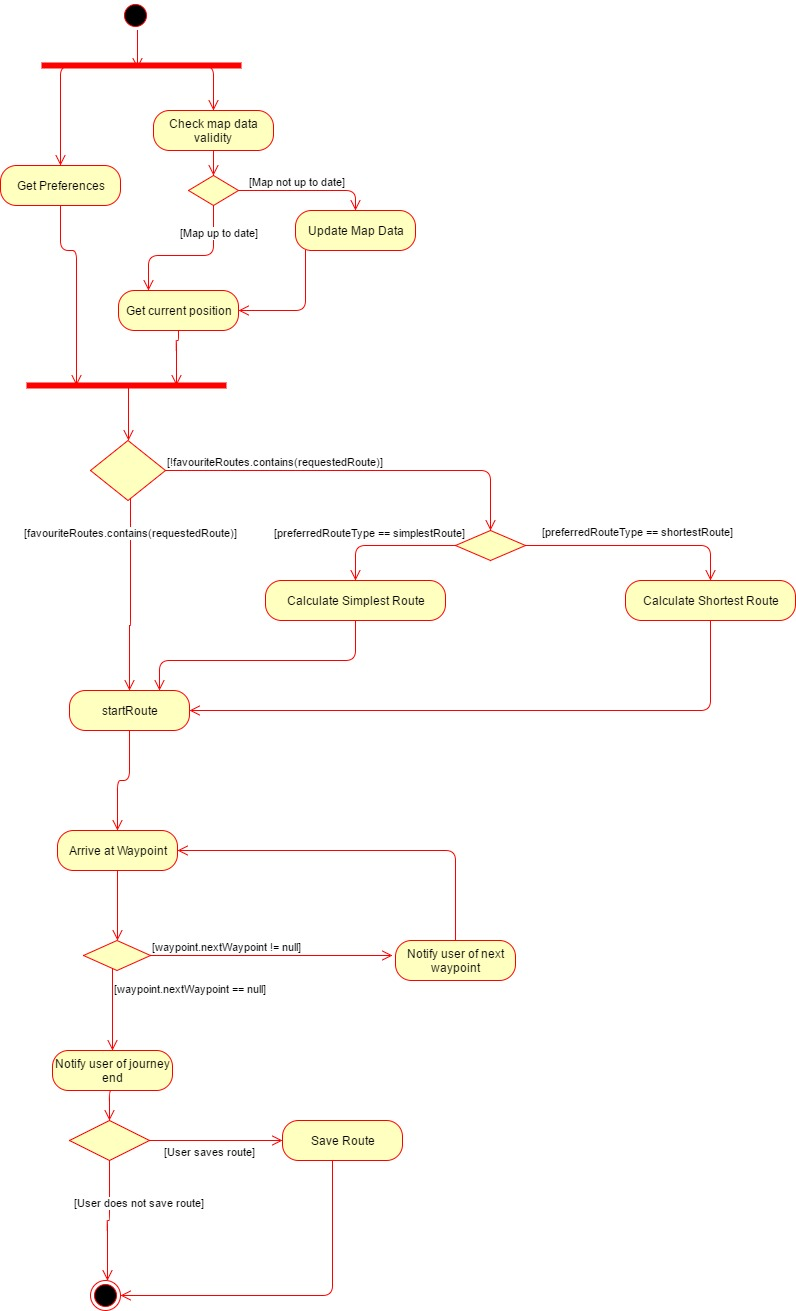
\includegraphics[width=\textwidth]{Navigation_Activity_Diagram}
        	\caption{Navigation Module Activity Diagram}
        \end{figure}
    \subsection{Points-of-interest}
    
        \subsubsection{Class Diagram}
	
	  \begin{figure} [!h]
            \centering
            \includegraphics[width = \textwidth, height = "15cm" ]{new_points_of_interest_class_diagram}
            \caption{Points of Interest Class Diagram}
            \label{Points of Interest Class Diagram}
        \end{figure}
	
        \subsubsection{Use Case Diagram}
	
	 \begin{figure} [!h]
            \centering
            \includegraphics[width = \textwidth, height = "15cm" ]{points_of_interest_use_case_diagram}
            \caption{Points of Interest Use Case Diagram}
            \label{Points of Interest Use Case Diagram}
        \end{figure}
	
        \subsubsection{Chosen Design Patterns}
	 For the Points of Interest Class Diagram the Factory and Facade design patterns are used. The Facade design pattern provides a 	 unified interface to a set of interfaces in the Points of Interest subsystem. The Facade defines a higher-level interface for 		 the Points of Interest that makes the subsystem easier to use. Thus it wraps a complicated subsystem with a simpler interface. 	 The Factory design pattern provides an interface for creating families of related or dependent objects without specifying their 	  concrete classes.
	 
\section{Technology Choices}
\subsection{Application Server}
The application server is the component responsible for hosting the business process layer of the NavUP system. It needs to be able to satisfy quality requirements mentioned in System Software Attributes section. The NavUP system will follow a layered reference architecture approached as well as implement a Services-Oriented Architecture(SOA) approach. Together they allow the system to be flexible, easily maintainable and easily deployable. \\[0.2cm]
JavaEE (Java Platform, Enterprise Edition) architecture is is one of the most widely used
reference architectures for large, interactive enterprise systems.JavaEE supports, amongst other things, standard access channels for enterprise systems, a solid process execution environment, a range of standard integration channels, hot deployment and clustering. The main aim is to provide a reference architecture for scalable, reliable, deploy-ability, flexibility and modularity. \\[0.2cm]
The application server will run on Tomcat 8 which is an open-source Java Servlet Container which offers great support for the JavaEE. It allows for easy deployment and modularity. Using the Web Services API it also interacts well with other technologies. 
\subsection{Database}
The system has strict scalability, reliability and flexibility quality requirements to satisfy. Many users will be connected to the system at the same time and the DBMS (Database Management System) needs to be reliable. It is important that a DBMS is chosen for which both the scalability and reliability requirements can be met. For this reason the system will use \textit{PostgreSQL} which is a reliable object-relational database. \\[0.2cm]
The NavUP system also needs to have a database to satisfy the requirements of the GIS subsystem for this purpose \textit{PostGIS} will be used. It is a spatial database extender for\textit{PostgresSQL}, so it adds support for geographical objects.  \\[0.2cm]
Both \textit{PostgreSQL} and \textit{PostGIS} have great JavaEE support through the use of a persistence API. They also have great community support.
\subsection{Persistence API}
The persistence API is middleware that provides a layer of abstraction between the  persistence provider (database) and the application. It is separated from the database technology as well as the  database selected for the system. Java EE offers JPA as its persistence API. JPA is considered as a standard approach for Object to Relational Mapping (ORM) in Java.\\ [0.2cm]
JavaEE again is a great choice to carry out the requirements of this system.

\subsection{Web Services Framework}
The web services framework is a wrapping layer of the application services (business processes) layer making the system services available over the Internet. This allows the application server to be separated from user-interface technologies.The web services framework should be based on a public standard and open-source implementation should be available.\\[0.2cm]
For the web services framework the project will use the Jersey implementation of the JAX-RS provided by JavaEE. A RESTful approach will be used.
\subsection{Mobile Application Frameworks}	
The system does not have any particular mobile OS requirement, for this purpose a hybrid mobile application framework will be used to build the mobile interface part of the system.\\[0.2cm]
 \textit{Ionic 2} is hybrid mobile application development framework build on top of Angular and Apache Cordova. \textit{Ionic 2} provides tools and services for developing hybrid mobile applications using web technologies like CSS, HTML5 and SASS. Since the NavUP system is going to be designed for both iOS and Android smartphones, \textit{Ionic 2} is the best fit framework to develop the mobile application. \\[0.2cm]
	It uses MVC (Model, View and Controller) architectural pattern which separates logical concerns.\\[0.2cm]
	\textbf{Other Frameworks Considered}\\ 
	\begin{enumerate}
		\item \textbf{PhoneGap} : Very old and outdated compared to Ionic
		\item \textbf{NativeScript} : still new and has less community support
	\end{enumerate}

\subsection{Web Application Framework}
 The web application architecture will be built using\textit{Angular}. \textit{Angular} is a rewrite of \textit{AngularJS} which is based on the MVVM and MVC architectures. \\
	
 \textbf{Other Frameworks Considered}\\ 
	\begin{enumerate}
		\item EmberJS 
		\item ReactJS
	\end{enumerate}

	

\end{document}
